\documentclass{article}
\usepackage{tikz}
\usetikzlibrary{arrows.meta, calc, positioning}

\begin{document}

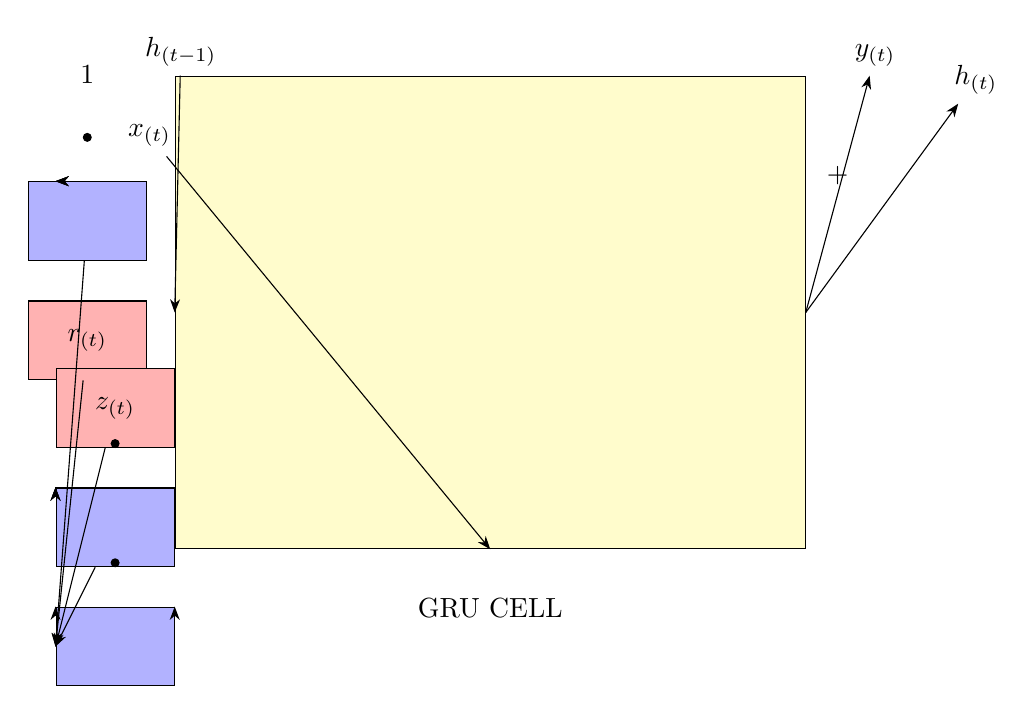
\begin{tikzpicture}[node distance=0.5cm, >=Stealth,
    cell/.style={draw, fill=yellow!20, minimum width=8cm, minimum height=6cm},
    fc/.style={draw, fill=blue!30, minimum width=1.5cm, minimum height=1cm},
    fc2/.style={draw, fill=red!30, minimum width=1.5cm, minimum height=1cm},
    dot/.style={circle, draw, inner sep=1pt, fill=black}
]

% Draw the cell
\node[cell] (cell) {};

% Input from previous time step
\node[left=of cell.north west, anchor=south west] (h_t_minus_1) {$h_{(t-1)}$};

% Input from current time step
\node[below=of h_t_minus_1, anchor=north east] (x_t) {$x_{(t)}$};

% Output from current time step
\node[right=of cell.north east, anchor=south west] (y_t) {$y_{(t)}$};
\node[right=of y_t, anchor=north west] (h_t) {$h_{(t)}$};

% Gates
\node[fc2, below left=of cell.west, anchor=east] (r_t) {$r_{(t)}$};
\node[fc2, below right=of r_t, anchor=east] (z_t) {$z_{(t)}$};

% Forget gate
\node[fc, above=of r_t, anchor=south] (forget_gate) {};
\node[dot, above=of forget_gate, anchor=south] (dot_forget) {};
\node[above=of dot_forget, anchor=south] (forget_label) {1};

% Update gate
\node[fc, below=of z_t, anchor=north] (update_gate) {};
\node[dot, above=of update_gate, anchor=south] (dot_update) {};
\node[above=of dot_update, anchor=south] (update_label) {};

% Cell state
\node[fc, below=of update_gate, anchor=north] (cell_state) {};
\node[dot, above=of cell_state, anchor=south] (dot_cell) {};
\node[above=of dot_cell, anchor=south] (cell_label) {};

% Connections
\draw[->] (h_t_minus_1) -- (cell.west);
\draw[->] (x_t) -- (cell.south);
\draw[->] (cell.east) -- node[above] {$+$} (y_t);
\draw[->] (cell.east) -- (h_t);

\draw[->] (r_t) -- (cell_state.west);
\draw[->] (z_t) -- (cell_state.west);

\draw[->] (forget_gate) -- (cell_state.west);
\draw[->] (update_gate) -- (cell_state.west);

\draw[->] (cell_state) -- (cell_state.north -| cell_state.west);
\draw[->] (cell_state) -- (cell_state.north -| cell_state.east);

\draw[->] (forget_gate) -- (forget_gate.north -| cell_state.west);
\draw[->] (update_gate) -- (update_gate.north -| cell_state.west);

\draw[->] (forget_gate) -- (forget_gate.north -| cell_state.west);
\draw[->] (update_gate) -- (update_gate.north -| cell_state.west);

\draw[->] (forget_gate) -- (forget_gate.north -| cell_state.west);
\draw[->] (update_gate) -- (update_gate.north -| cell_state.west);

\node[below=of cell, anchor=north] (gru_cell) {GRU CELL};

\end{tikzpicture}

\end{document}